\chapter{triangular\_shelf}

\section{Purpose}

To compare \telemac{2D} simulation with a benchmark
(\url{http://isec.nacse.org/workshop/2009_isec/benchmarks.html#bmark1}).

\section{Description}

The configuration is a 48.8~m long and 26.5~m wide rectangle.
Water Depth is 0.78~m.

\subsection{Geometry and mesh}

Figure~\ref{fig:triang:geometry} shows the geometry of the study.

\begin{figure}[H]
\centering
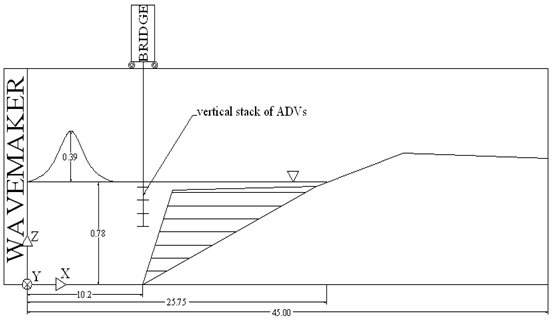
\includegraphics[width=.6\textwidth]{img/geom.png}
\caption{Geometry of the study.}
\label{fig:triang:geometry}
\end{figure}

The mesh is made of 36,874 elements and 18,720 nodes,
see Figure~\ref{fig:triang:mesh}.

\begin{figure}[H]
\centering
\includegraphicsmaybe{[width=.6\textwidth]}{../img/Mesh.png}
\caption{Mesh of the study.}
\label{fig:triang:mesh}
\end{figure}

Figure~\ref{fig:triang:bathy} shows the bathymetry of the study.

\begin{figure}[H]
\centering
\includegraphicsmaybe{[width=.6\textwidth]}{../img/Bathy.png}
\caption{Bathymetry of the study.}
\label{fig:triang:bathy}
\end{figure}

\subsection{Boundaries}

Figure~\ref{fig:triang:boundaries} shows the boundaries of the study.

\begin{figure}[H]
\centering
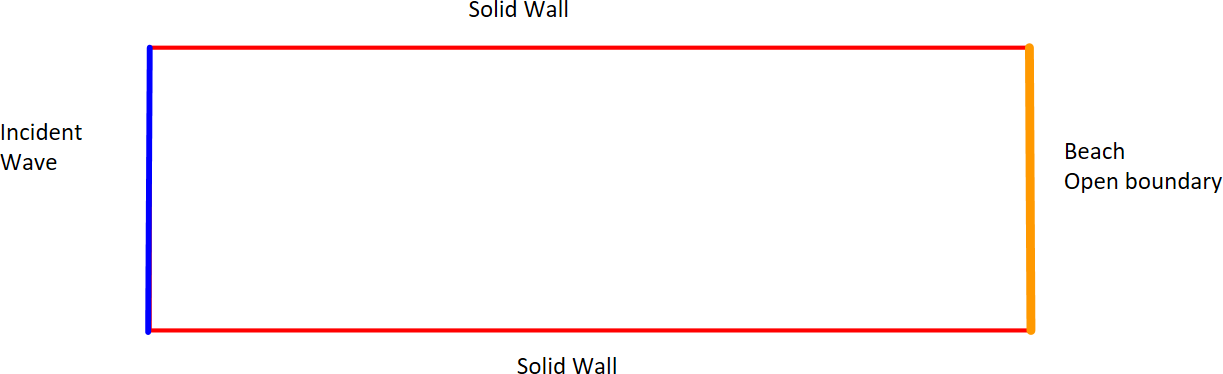
\includegraphics[width=.6\textwidth]{img/boundaries.png}
\caption{Geometry of the study.}
\label{fig:triang:boundaries}
\end{figure}

Single solitary wave generated ($H$ = 0.39~m)

Bottom:
\begin{itemize}
  \item Chezy's Law,
  \item Friction coefficient: 180~m$^{1/2}$/s.
\end{itemize}

\subsection{Physical parameters}

Turbulence: Constant viscosity equal to zero.

\subsection{Numerical parameters}

\begin{itemize}
  \item Type of element: P1 triangle for $h$ and for velocity,
  \item Solver: GMRES,
  \item Accuracy: $10^{-6}$,
  \item Finite volume scheme: Kinetic order 2.
\end{itemize}

\begin{table}[H]
  \begin{center}

    \begin{tabular*}{.9\textwidth}{|c|c|c|}
  \hline
  Equations & Saint-Venant VF & Boussinesq \\
  Time step & 0.05 & 0.005 \\
  Simulation duration & 20 & 20 \\
  \hline
\end{tabular*}
  \end{center}
\end{table}

\section{Results}
We compare the model and experiment free surface at
\begin{itemize}
  \item $X$ = 25~m,
  \item $Y$ =  0~m,
  \item $Y$ = -5~m.
\end{itemize}

Figure~\ref{fig:triang:vel} shows the velocity vectors.

\begin{figure}[H]
\centering
\includegraphicsmaybe{[width=.9\textwidth]}{../img/FreeSurface.png}
%The time step of this fixed figure is greater than the duration of the current simulation
%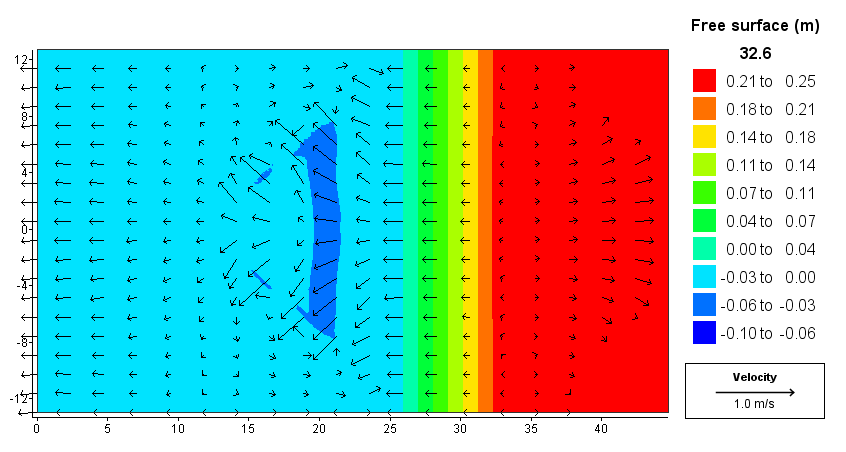
\includegraphics[width=.6\textwidth]{img/vel.png}
\caption{Velocity vectors over the free surface.}
\label{fig:triang:vel}
\end{figure}

Figure~\ref{fig:triang:res} shows the comparison with the benchmark data.

\begin{figure}[H]
\centering
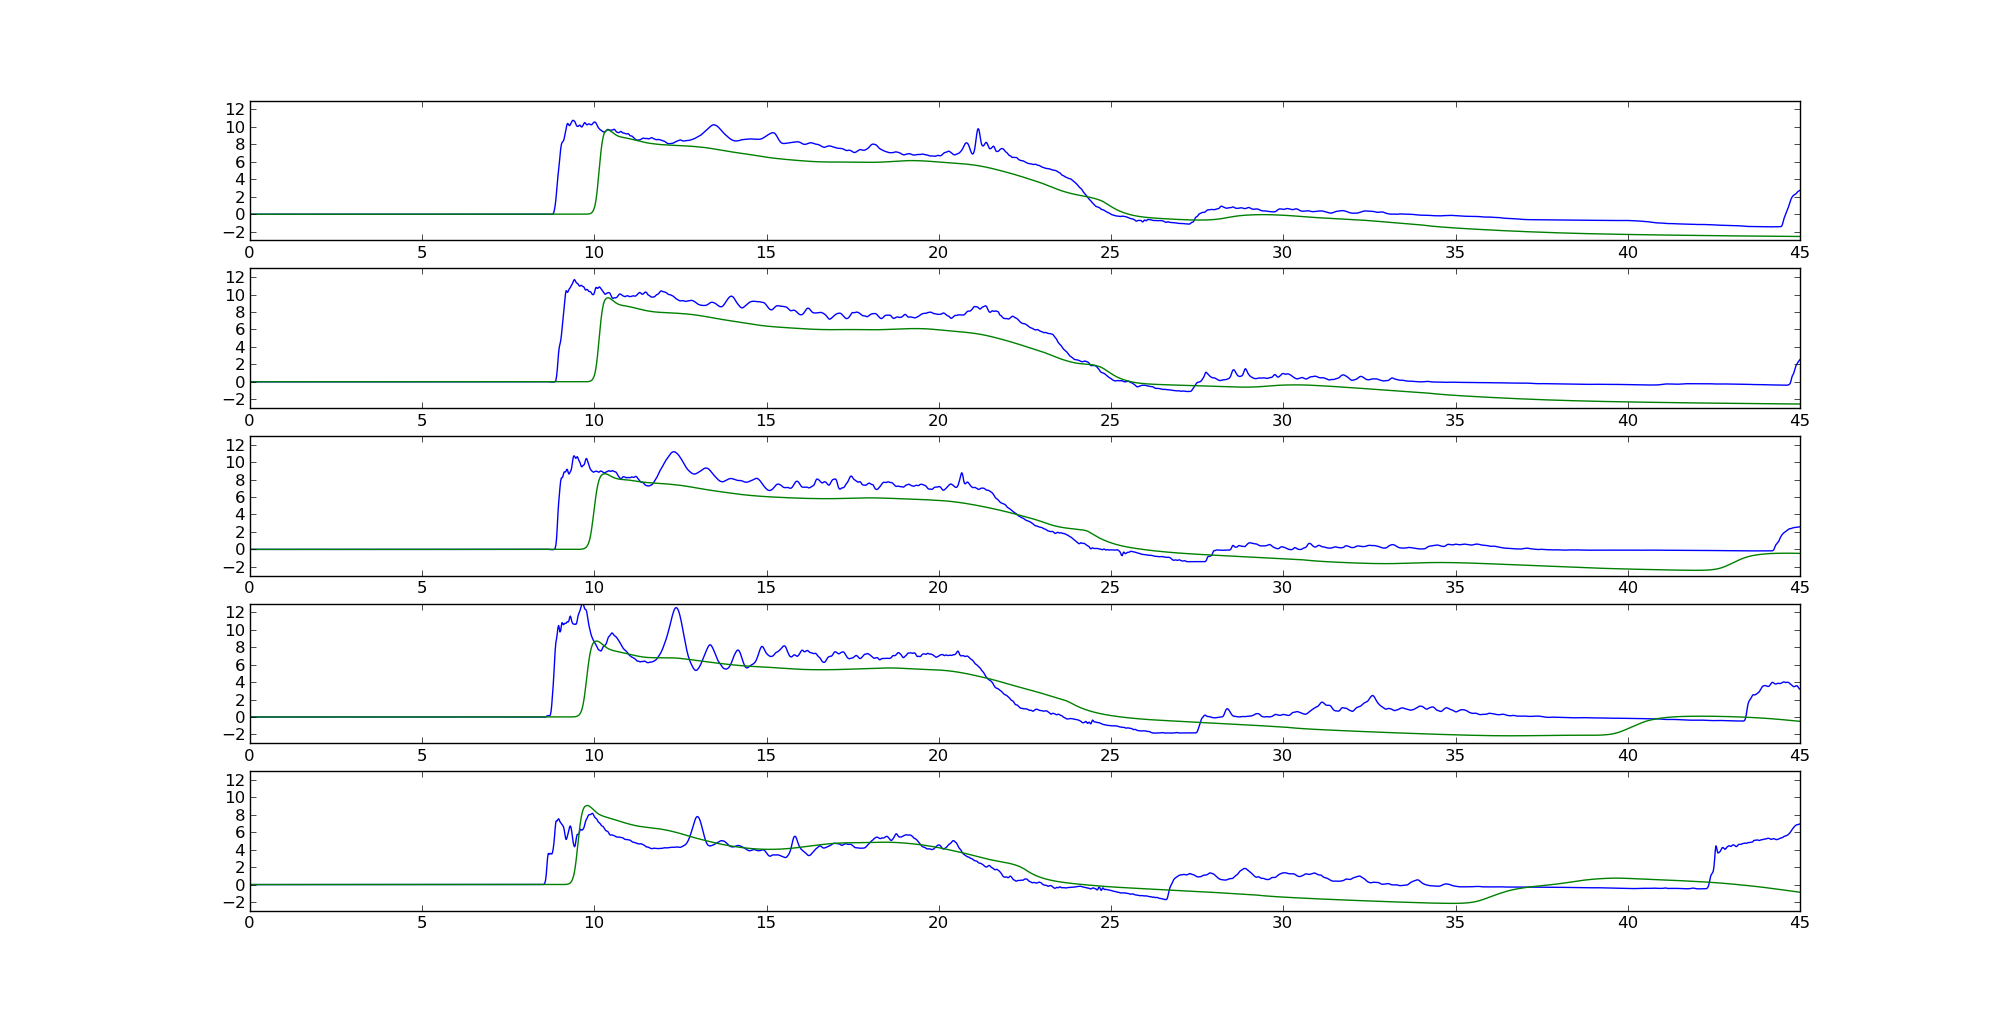
\includegraphics[width=.8\textwidth]{img/res_X25.png}
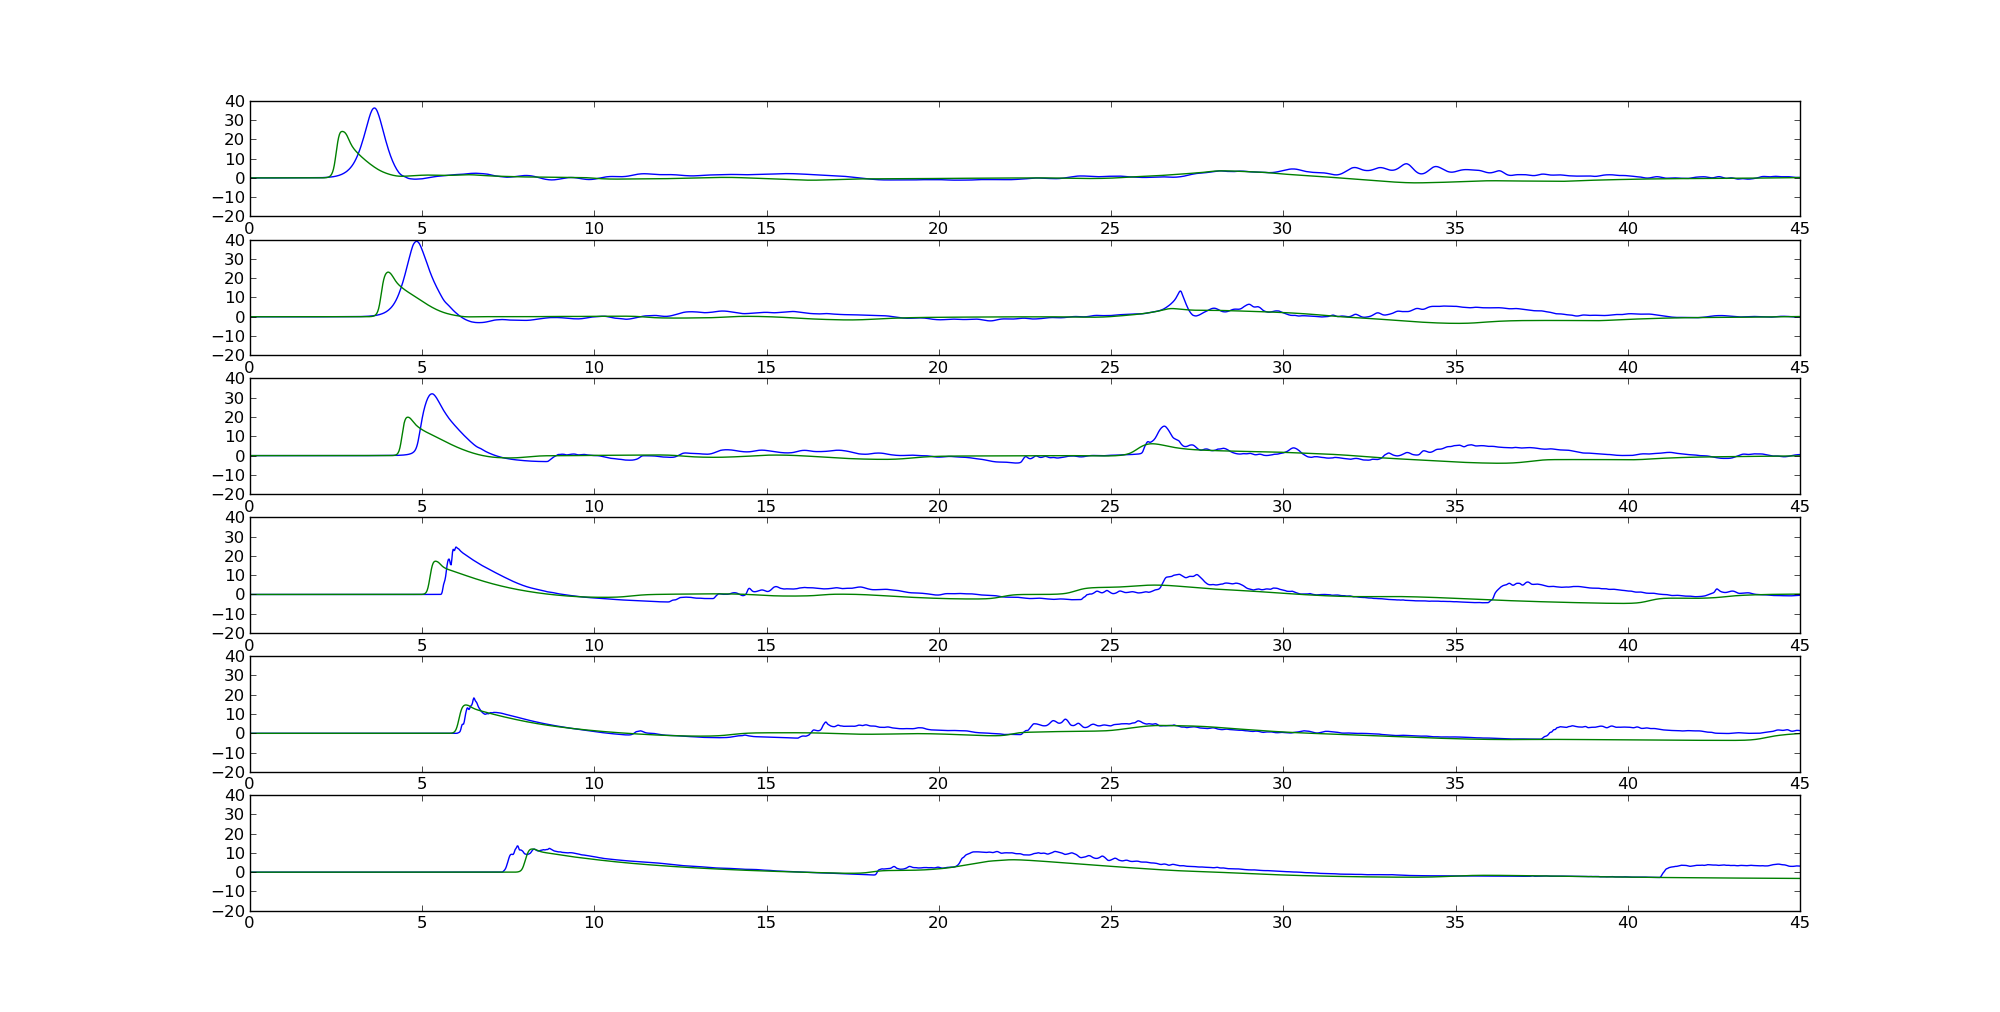
\includegraphics[width=.8\textwidth]{img/res_Y0.png}
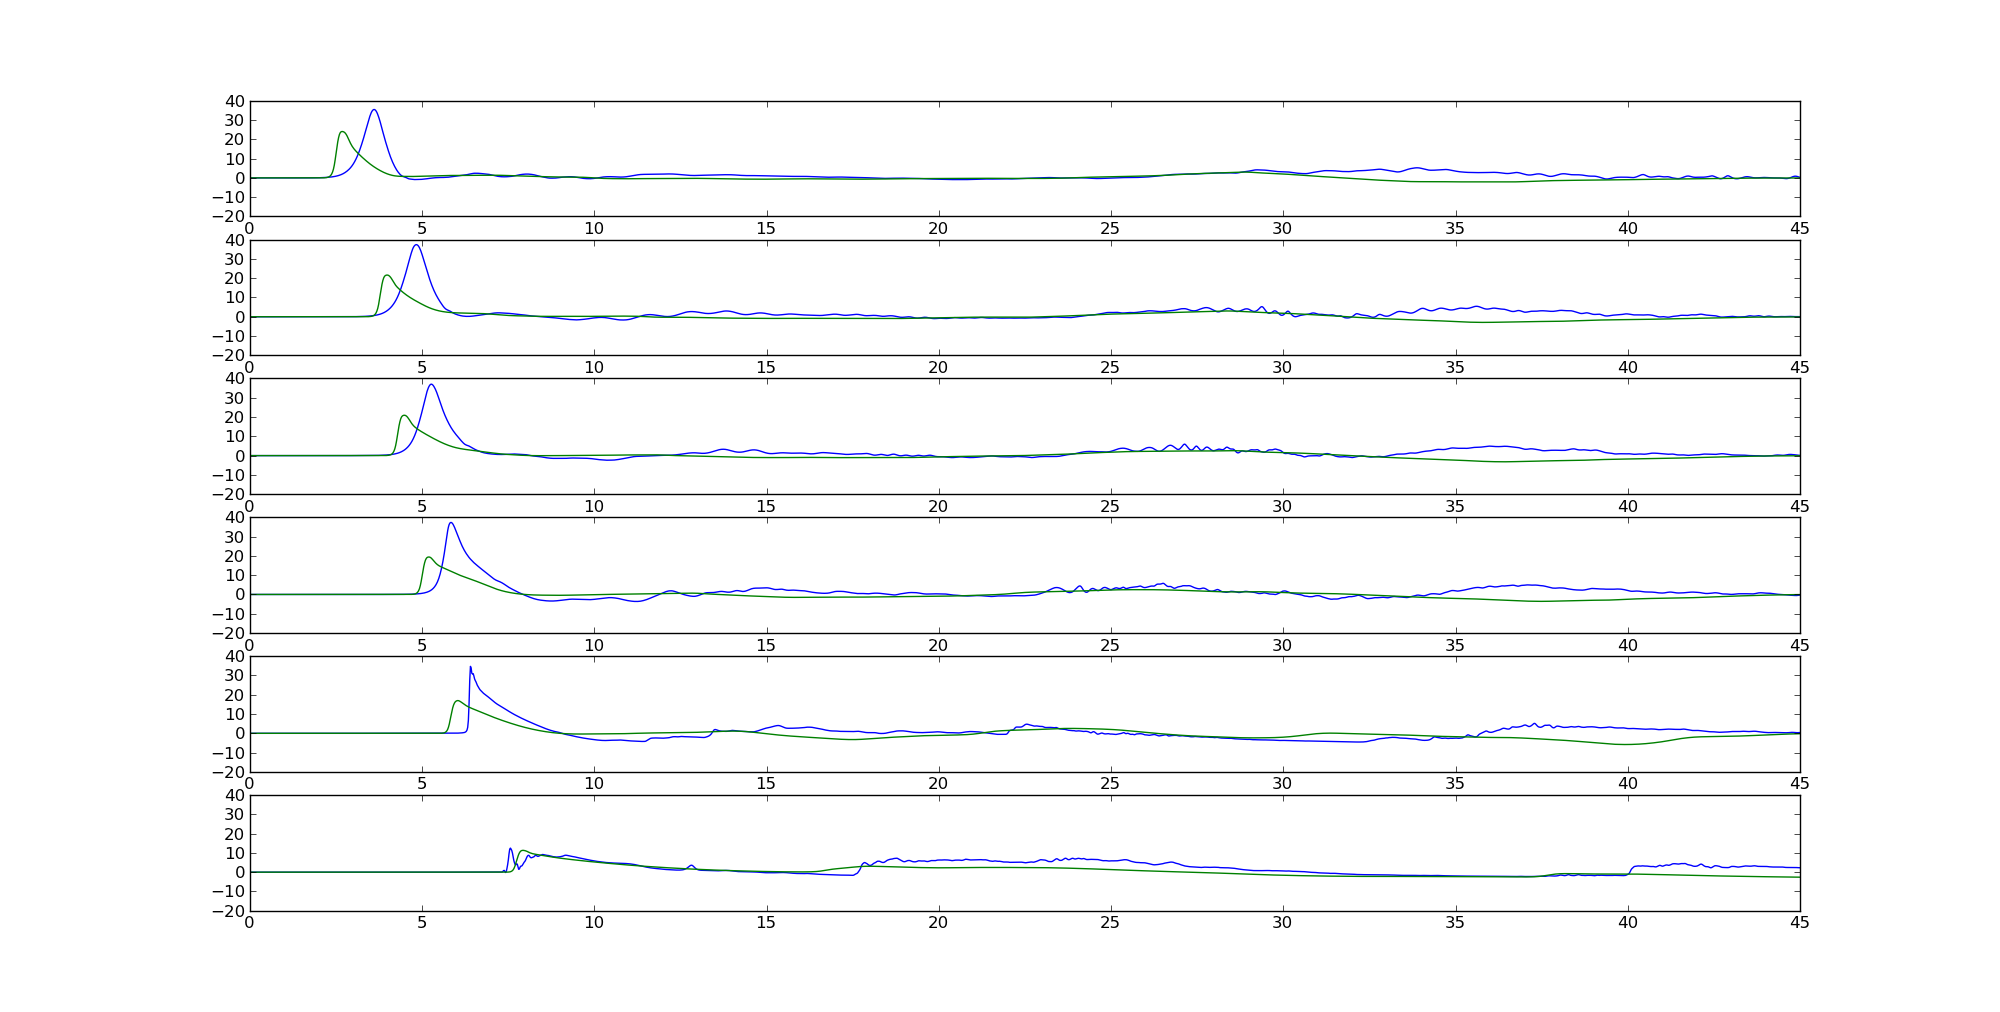
\includegraphics[width=.8\textwidth]{img/res_Y-5.png}
\caption{Comparaison of the results: in blue the experiment and in green the model.}
\label{fig:triang:res}
\end{figure}
